\documentclass{article}

\usepackage[main]{neurips_2026}

\usepackage[utf8]{inputenc}
\usepackage[T1]{fontenc}
\usepackage{hyperref}
\usepackage{url}
\usepackage{booktabs}
\usepackage{amsfonts}
\usepackage{amsmath}
\usepackage{amssymb}
\usepackage{amsthm}
\usepackage{nicefrac}
\usepackage{microtype}
\usepackage{xcolor}
\usepackage{graphicx}
\usepackage{algorithm}
\usepackage{algorithmic}
\usepackage[textsize=tiny, textwidth=2cm]{todonotes}
\setlength{\marginparwidth}{2cm}
\usepackage{listings}

\newtheorem{theorem}{Theorem}
\newtheorem{proposition}[theorem]{Proposition}
\newtheorem{lemma}[theorem]{Lemma}
\newtheorem{corollary}[theorem]{Corollary}
\newtheorem{definition}[theorem]{Definition}
\newtheorem{remark}[theorem]{Remark}

\DeclareMathOperator{\tr}{tr}
\DeclareMathOperator{\diag}{diag}
\DeclareMathOperator{\vect}{vec}
\newcommand{\R}{\mathbb{R}}
\newcommand{\C}{\mathbb{C}}
\newcommand{\Z}{\mathbb{Z}}
\newcommand{\fhat}{\hat{f}}
\newcommand{\Fhat}{\hat{F}}
\newcommand{\betasel}{\beta^{\mathrm{sel}}}
\newcommand{\betafull}{\beta^{\mathrm{full}}}
\newcommand{\SO}{\mathrm{SO}}
\newcommand{\OG}{\mathrm{O}}

\lstset{
  language=Python,
  basicstyle=\ttfamily\small,
  keywordstyle=\color{blue},
  commentstyle=\color{gray},
  stringstyle=\color{red},
  frame=single,
  breaklines=true,
  columns=fullflexible,
}

\title{\texttt{bispectrum}: Selective $G$-Bispectra Made Practical}

\author{%
  Johan Mathe \\
  Atmo, Inc. \\
  \texttt{johan@atmo.ai} \\
  \And
  Nina Miolane \\
  University of California, Santa Barbara \\
  \texttt{nmiolane@ucsb.edu} \\
}

\begin{document}

\maketitle

\begin{abstract}
\todo[inline]{Write abstract ($\sim$150 words). Key points to hit:}
\begin{itemize}
  \item We release \texttt{bispectrum}, the first PyTorch library for computing
    selective $G$-bispectra---the unique complete and exact group-invariant
    features, with $O(|G|)$ coefficients for finite groups.
  \item The library supports 7 group/domain pairs
    ($C_n$, $D_n$, $O$, $\SO(2)/S^1$, $\SO(2)/\text{disk}$,
    $\SO(3)/S^2$, torus) as differentiable \texttt{nn.Module}s with GPU
    acceleration, signal inversion, and applications to invariant pooling,
    orbit-invariant regularization, and multi-reference alignment.
  \item Building the library required solving two open engineering challenges:
    bridging steerable CNN features to group Fourier coefficients for
    non-abelian groups (Theorem~\ref{thm:steerable-fourier}), and
    resolving a previously undocumented inversion failure for the
    octahedral group via bootstrap + Levenberg--Marquardt.
  \item On PatchCamelyon, bispectral pooling achieves the highest AUC
    among equivariant nonlinearities, the most stable accuracy--parameter
    Pareto frontier across architectures, and near-perfect rotation
    invariance. On RotMNIST, a bispectral contrastive regularizer
    improves rotation robustness.
  \item The library is pip-installable, MIT-licensed, and integrates
    into standard PyTorch training pipelines.
\end{itemize}
\end{abstract}


\section{Introduction}
\label{sec:intro}

\todo[inline]{Write introduction ($\sim$1 page). Follow the narrative arc below.}

\paragraph{The invariant nonlinearity bottleneck.}
Equivariant convolutional neural networks~\citep{cohen2016group, weiler2019general}
achieve symmetry by design, replacing data augmentation with group convolutions that
guarantee equivariant feature maps. Yet every such architecture must eventually
produce \emph{invariant} features---for classification, regression, or any
prediction that should not depend on input orientation.
The choice of invariant map is a critical design decision with no consensus
solution (Table~\ref{tab:nonlinearity-comparison}).
Existing approaches sacrifice either completeness (norm, gate), exactness
(Fourier pointwise), or efficiency (tensor product, full bispectrum).

\begin{table}[h]
  \caption{Invariant nonlinearities for equivariant CNNs. The selective bispectrum,
    implemented in our library, is the only method that is simultaneously exact,
    complete, and linear-cost for finite groups.}
  \label{tab:nonlinearity-comparison}
  \centering
  \small
  \begin{tabular}{lcccc}
    \toprule
    Nonlinearity & Exact? & Complete? & Coefficients & Key limitation \\
    \midrule
    Norm          & Yes & No  & $O(|G|)$      & Discards phase \\
    Gate          & Yes & No  & $O(2|G|)$     & Scalar bottleneck \\
    Fourier pointwise & No & Yes & $O(|G| \log |G|)$ & Aliasing \\
    Tensor product & Yes & Yes & $O(|G|^3)$   & Cubic cost \\
    Full bispectrum & Yes & Yes & $O(|G|^2)$  & Quadratic cost \\
    \midrule
    \textbf{Sel.\ bispectrum} & \textbf{Yes} & \textbf{Yes} & $\mathbf{O(|G|)}$$^\dagger$ & \textbf{(this work)} \\
    \bottomrule
  \end{tabular}

  \vspace{0.3em}
  {\small $^\dagger$For finite groups where selectivity is
    proven~\citep{mataigne2024selective}. Selective $\SO(3)$ on $S^2$
    remains open.}
\end{table}

\paragraph{The gap from theory to practice.}
The selective $G$-bispectrum~\citep{mataigne2024selective} provides $O(|G|)$-cost
complete invariants for finite groups, and \citet{myers2025selective} extend this
to the disk. However, no practical software exists. Moving from theorems to a
usable library required solving three problems:
\begin{enumerate}
  \item No GPU-accelerated implementation exists for any group beyond toy examples.
  \item For the octahedral group, the theoretically prescribed bootstrap inversion
    algorithm fails due to an $\SO(3)$ phase ambiguity not addressed by the
    Clebsch--Gordan structure (Section~\ref{sec:lib-octa}).
  \item Steerable CNN feature maps live in intertwiner spaces, not in group Fourier
    spaces---for non-abelian groups, one cannot na\"ively plug steerable outputs
    into the bispectrum formula (Section~\ref{sec:lib-steerable}).
\end{enumerate}

\paragraph{Contributions.}
We present \texttt{bispectrum}, a PyTorch library that makes selective
$G$-bispectra practical as differentiable primitives for invariant feature
extraction, regularization, and signal reconstruction:
\begin{enumerate}
  \item \textbf{\texttt{bispectrum} library} (Section~\ref{sec:library}):
    The first PyTorch library for selective $G$-bispectra, supporting
    7 group/domain pairs as \texttt{nn.Module}s with GPU acceleration,
    signal inversion, and seamless integration into training pipelines.
    Beyond invariant pooling, the library enables orbit-invariant losses,
    metric learning, and multi-reference alignment
    (Section~\ref{sec:lib-beyond}).
    Pip-installable, MIT-licensed, with CI/CD and $>$90\% test coverage.

  \item \textbf{Engineering contribution: steerable-to-Fourier bridge}
    (Section~\ref{sec:lib-steerable}):
    We prove conditions under which steerable convolution outputs yield valid
    group Fourier coefficients for bispectral computation
    (Theorem~\ref{thm:steerable-fourier}), enabling integration with
    existing equivariant architectures.

  \item \textbf{Engineering contribution: octahedral inversion}
    (Section~\ref{sec:lib-octa}):
    We identify a previously undocumented inversion failure for the octahedral
    group and resolve it via bootstrap initialization followed by
    Levenberg--Marquardt refinement.

  \item \textbf{Empirical validation} (Section~\ref{sec:experiments}):
    On PatchCamelyon, bispectral pooling achieves the highest AUC among
    equivariant nonlinearities, the flattest accuracy--parameter Pareto
    frontier (most robust to architecture choices), and near-perfect
    rotation invariance ($\sigma_{\text{AUC}} < 0.002$).
    On RotMNIST, a bispectral contrastive regularizer improves rotation
    robustness without augmentation labels.
    \todo[inline]{Update RotMNIST claim once experiment is run.}
\end{enumerate}


\section{Mathematical Preliminaries}
\label{sec:preliminaries}

\subsection{Equivariant CNNs and invariant maps}
\label{sec:prelim-equiv}

\todo[inline]{Write $\sim$0.5 page on equivariant CNNs. Cover:}
\begin{itemize}
  \item Group convolutions: a convolution layer is $G$-equivariant if
    $[\pi(g) \circ \Phi](f) = \Phi(\pi(g) f)$ for all $g \in G$.
    Cite \citet{cohen2016group}.
  \item Regular vs.\ steerable representations. In regular representations,
    features are functions $f: G \to \R^C$. In steerable representations,
    features transform as $f \mapsto \rho(g) f$ for a representation
    $\rho$~\citep{weiler2019general}.
  \item The need for $G$-invariant pooling: to produce predictions
    that do not depend on the input orientation, one must map equivariant
    features to invariant ones.
  \item Existing invariant maps: norm (discards phase), gated nonlinearity
    (scalar bottleneck), Fourier pointwise (approximate equivariance due to
    aliasing~\citep{franzen2021general}), tensor product / CG product
    ($O(L^3)$ cost~\citep{kondor2018clebsch}).
\end{itemize}


\subsection{The $G$-bispectrum}
\label{sec:prelim-bispectrum}

\todo[inline]{Write $\sim$0.5 page. Merge the G-bispectrum definition and selective bispectra into one subsection. Cover:}
\begin{itemize}
  \item Group Fourier transform: for a finite group $G$ with irreducible
    representations $\{\rho_i\}_{i \in \hat{G}}$,
    \begin{equation}
      \Fhat(\rho_i) = \sum_{g \in G} f(g)\, \rho_i(g) \in \C^{d_i \times d_i}.
    \end{equation}
  \item The $G$-bispectrum: given the Clebsch--Gordan decomposition
    $\rho_i \otimes \rho_j \cong \bigoplus_k m_{ij}^k \rho_k$
    with intertwining matrix $C_{ij}$,
    \begin{equation}
      \label{eq:bispectrum-def}
      \beta_{\rho_i, \rho_j} = C_{ij}^\top\,
        (\Fhat(\rho_i) \otimes \Fhat(\rho_j))\,
        C_{ij}\, \Fhat(\rho_k)^\dagger.
    \end{equation}
  \item Completeness: the bispectrum is a \emph{complete} invariant---it
    separates orbits under the $G$-action~\citep{kakarala1992triple}.
  \item Full cost: $O(|G|^2)$ coefficients for finite groups.
  \item \textbf{Selective bispectra}~\citep{mataigne2024selective}: for finite groups,
    $O(|G|)$ bispectral coefficients suffice for completeness, selected via a
    BFS on the Kronecker product table of $\hat{G}$. The disk
    extension~\citep{myers2025selective} gives $O(N)$ Fourier--Bessel
    coefficients for $\SO(2)$-invariance on the unit disk.
  \item Bootstrap inversion algorithms recover $f$ (up to group action) from
    the selective bispectrum for commutative and dihedral groups.
\end{itemize}


\subsection{The representation-theoretic gap}
\label{sec:prelim-gap}

\todo[inline]{Write $\sim$0.3 page briefly identifying the steerable gap. This motivates Section~\ref{sec:lib-steerable}. Cover:}
\begin{itemize}
  \item Steerable convolution outputs transform as $f \mapsto \rho(g) f$
    where $\rho$ is a (potentially reducible) representation.
  \item For abelian groups ($C_n$, $\SO(2)$): all irreps are 1D characters,
    so intertwiner coefficients \emph{are} Fourier coefficients. No gap.
  \item For non-abelian groups ($D_n$, $O$): the intertwiner space
    $\mathrm{Hom}_G(\rho_i, \rho_{\text{out}})$ has dimension
    $m_i = \text{multiplicity of } \rho_i \text{ in } \rho_{\text{out}}$.
    When $m_i < d_i$ (the dimension of $\rho_i$), steerable outputs do not
    span the full Fourier matrix---one cannot na\"ively apply the bispectrum
    formula.
  \item Concrete example: for $D_4$ with output type $\rho_1 \oplus \rho_0$,
    the steerable features give only 3 numbers but the Fourier transform of
    $\rho_1$ needs $2^2 = 4$.
  \item We solve this within the library (Section~\ref{sec:lib-steerable}).
\end{itemize}


\section{The \texttt{bispectrum} Library}
\label{sec:library}

This section describes the design, scope, and key engineering contributions
of the \texttt{bispectrum} library. Following the structure advocated by
\citet{paszke2019pytorch} and \citet{gardner2018gpytorch}, we focus on
\emph{design principles and trade-offs} rather than a usage tutorial.

\subsection{Design principles}
\label{sec:lib-design}

\todo[inline]{Write $\sim$0.5 page on design principles. Frame as a \emph{design manifesto} (per PyTorch Reviewer 2's advice). Cover:}
\begin{itemize}
  \item \textbf{P1: Naming encodes the math.} Class names follow
    \texttt{\{Group\}on\{Domain\}} (e.g., \texttt{CnonCn},
    \texttt{SO3onS2}, \texttt{SO2onDisk}). A reader unfamiliar with the
    codebase immediately identifies the group and domain from the class name.
    This is deliberately mathematical rather than verbal
    (\texttt{CyclicBispectrum}) because the mathematical name carries
    precise meaning and scales as the library grows.

  \item \textbf{P2: \texttt{nn.Module} only.} Every bispectrum computation
    is a \texttt{torch.nn.Module} subclass. No parallel functional API.
    One way to compute a bispectrum. Precomputed quantities
    (CG matrices, DFT kernels, Bessel roots) are registered as
    non-learnable buffers, so \texttt{.to(device)} and \texttt{.to(dtype)}
    work transparently.

  \item \textbf{P3: Selective by default.} All modules default to
    \texttt{selective=True}, computing the minimal $O(|G|)$ coefficient set.
    The full $O(|G|^2)$ bispectrum is available via \texttt{selective=False}
    for debugging and comparison.

  \item \textbf{P4: Raw signals in.} Modules accept real-valued signals
    in the natural domain (spatial grid, discrete cycle, sphere) and handle
    the Fourier transform internally. For example, \texttt{SO3onS2} accepts
    signals of shape $(B, n_{\text{lat}}, n_{\text{lon}})$ and computes
    the spherical harmonic transform internally. This keeps the interface
    clean and prevents Fourier-convention mismatches.

  \item \textbf{P5: Inversion on-module.} Every module exposes
    \texttt{bsp.invert(beta)} that returns the reconstructed signal
    (up to group-action indeterminacy) or raises a precise
    \texttt{NotImplementedError} with guidance.

  \item \textbf{P6: Minimal dependencies.} The library depends only on
    \texttt{torch} and \texttt{numpy}. No external CG library:
    Clebsch--Gordan matrices for $D_n$ are computed analytically,
    for $\SO(3)$ they are bundled as pre-computed JSON, and Bessel roots
    for the disk are computed via a pure-torch Newton-bisection solver
    using the interlacing property.
\end{itemize}


\subsection{Supported groups and API}
\label{sec:lib-groups}

Table~\ref{tab:supported-groups} lists all 7 group/domain pairs currently
supported by the library.

\begin{table}[h]
  \caption{Supported group/domain pairs in the \texttt{bispectrum} library.
    Selective coefficient counts are $O(|G|)$ vs.\ $O(|G|^2)$ for the full
    bispectrum. All modules share a uniform \texttt{nn.Module} interface.}
  \label{tab:supported-groups}
  \centering
  \small
  \begin{tabular}{llrrcc}
    \toprule
    Module & Group / Domain & Selective & Full & Inversion & Complexity \\
    \midrule
    \texttt{CnonCn}       & $C_n$ on $C_n$            & $n$    & $n^2$  & \checkmark & $O(n \log n)$ \\
    \texttt{SO2onS1}      & $\SO(2)$ on $S^1$         & $n$    & $n^2$  & \checkmark & $O(n \log n)$ \\
    \texttt{TorusOnTorus}  & $\prod C_{n_l}$ on torus  & $|G|$  & $|G|^2$ & \checkmark & $O(|G| \log |G|)$ \\
    \texttt{DnonDn}       & $D_n$ on $D_n$            & ${\sim}4|D_n|$ & ---  & \checkmark & $O(n)$ \\
    \texttt{OctaonOcta}   & $O$ on $\R^3$             & 172    & ---    & \checkmark$^*$ & $O(1)$ \\
    \texttt{SO3onS2}      & $\SO(3)$ on $S^2$         & ---    & $O(L^2)$ & ---       & $O(L^2 d_{\max}^2)$ \\
    \texttt{SO2onDisk}    & $\SO(2)$ on disk           & $N$    & $N^3$  & \checkmark & $O(N)$ \\
    \bottomrule
  \end{tabular}

  \vspace{0.3em}
  {\small $^*$Bootstrap + LM refinement (Section~\ref{sec:lib-octa}).}
\end{table}

\paragraph{Module interface contract.}
Every module satisfies: (i)~\texttt{forward(f)} accepts a real-valued signal
of shape $(B, \ldots)$ and returns a complex tensor of shape
$(B, \texttt{output\_size})$; (ii)~\texttt{output\_size} gives the number of
bispectral coefficients; (iii)~\texttt{index\_map} maps each flat output
index to its irrep index tuple $(\rho_i, \rho_j)$;
(iv)~no trainable parameters; (v)~deterministic output.

\paragraph{Usage examples.}

\begin{lstlisting}
import torch
from bispectrum import CnonCn, SO3onS2, SO2onDisk

# Cyclic group on Z/8Z: selective reduces 64 -> 8 coefficients
bsp = CnonCn(n=8, selective=True)
f = torch.randn(32, 8)              # batch of 32 signals
beta = bsp(f)                       # (32, 8), complex64
f_rec = bsp.invert(beta)            # (32, 8), up to cyclic shift

# SO(3) on the sphere
bsp_s2 = SO3onS2(lmax=5, nlat=64, nlon=128)
f_sphere = torch.randn(4, 64, 128)  # spherical signal
beta_s2 = bsp_s2(f_sphere)          # (4, output_size), complex64

# SO(2) on the unit disk
bsp_disk = SO2onDisk(L=16, selective=True)
f_disk = torch.randn(4, 16, 16)     # disk image
beta_disk = bsp_disk(f_disk)         # (4, N), complex128
f_rec = bsp_disk.invert(beta_disk)   # (4, 16, 16)
\end{lstlisting}


\subsection{Beyond invariant pooling}
\label{sec:lib-beyond}

Because every module is a differentiable \texttt{nn.Module} with both
\texttt{forward} and \texttt{invert}, the library supports use cases
beyond invariant feature extraction:

\paragraph{Orbit-invariant regularization.}
For generative or reconstruction tasks, the bispectrum provides a
rotation-invariant loss without augmentation: the loss
$\|\betasel(f_{\text{pred}}) - \betasel(f_{\text{target}})\|^2$ is
invariant to the $G$-action on both signals by construction.
We demonstrate this as a contrastive regularizer in
Section~\ref{sec:exp-contrastive}.

\paragraph{Orbit distance and metric learning.}
$\|\betasel(f) - \betasel(g)\|$ defines a distance between
signals modulo group action, suitable for retrieval, clustering, or
nearest-neighbor classification on equivalence classes.

\paragraph{Multi-reference alignment.}
Recovering a signal from noisy copies at unknown orientations reduces
to bispectral averaging followed by
inversion~\citep{myers2025selective, bendory2017bispectrum}.
The \texttt{invert()} method provides this primitive.

\paragraph{Symmetry detection.}
Vanishing patterns in bispectral coefficients reveal hidden symmetries
in data: a signal invariant to a subgroup $H \leq G$ produces a
bispectrum with predictable zero blocks.

\begin{lstlisting}
import torch
from bispectrum import CnonCn

bsp = CnonCn(n=8, selective=True)

# 1. Invariant features for classification
features = bsp(signal)               # (B, 8), complex64

# 2. Orbit-invariant regularization loss
loss = torch.nn.functional.mse_loss(bsp(pred).abs(), bsp(target).abs())

# 3. Signal reconstruction from bispectral coefficients
reconstructed = bsp.invert(features)  # (B, 8), up to cyclic shift
\end{lstlisting}


\subsection{Bridging steerable features to bispectra}
\label{sec:lib-steerable}

For abelian groups, steerable convolution outputs are directly usable as
Fourier coefficients, and the bispectrum formula applies out of the box.
For non-abelian groups ($D_n$, $O$), steerable outputs live in an
intertwiner space whose dimension does not match the number of irreps
(Section~\ref{sec:prelim-gap}). We resolve this mismatch:

\begin{theorem}[Steerable-to-Fourier bridge]
\label{thm:steerable-fourier}
  \todo[inline]{Insert the precise one-paragraph statement of P4 here.
    Conditions: output type contains each irrep $\rho_i$ with multiplicity
    $m_i \geq d_i$, or a multi-head architecture targets each irrep block.}
\end{theorem}

The proof and a detailed discussion of which \texttt{escnn} architectures
satisfy the theorem's conditions are in Appendix~\ref{app:proofs}.
In practice, this theorem justifies the \texttt{BispectrumPool} layer used
in our experiments (Section~\ref{sec:experiments}): extract Fourier
coefficients from the group dimension via the group DFT, compute the
selective bispectrum using the appropriate library module, log-compress
for numerical stability, and project back via a $1 \times 1$ convolution.


\subsection{Resolving the octahedral inversion gap}
\label{sec:lib-octa}

\todo[inline]{Write $\sim$0.5 page. Reframed as an engineering problem solved within the library. Cover:}

Implementing inversion for the octahedral group (\texttt{OctaonOcta}) revealed
a failure mode in the bootstrap algorithm of \citet{mataigne2024selective}:

\begin{itemize}
  \item The bootstrap recovers $\Fhat(\rho_1)$ up to an unknown
    $Q \in \SO(3)$. For $D_n$, the analogous $\OG(2)$ ambiguity is
    absorbed by CG matrices because $D_n$ irreps are restrictions of
    $\SO(2)$ irreps. For $O$, the CG matrix $C_{11}$ block-diagonalizes
    $\rho_1(g) \otimes \rho_1(g)$ only for $g \in O$, not for arbitrary
    $Q \in \SO(3)$.
  \item Numerically, $\|[C_{11}^\top (Q \otimes Q) C_{11}]_{\rho_2, \rho_3}\|_\infty
    \approx 0.788$ for generic $Q$---$O(1)$ cross-block leakage that
    corrupts the recovered Fourier coefficients.
  \item The selective $O$-bispectrum \emph{is} complete (172 coefficients
    uniquely determine the signal up to $O$-action). The failure is purely
    algorithmic: the sequential bootstrap cannot isolate individual Fourier
    blocks.
\end{itemize}

\paragraph{Resolution implemented in the library.}
\begin{enumerate}
  \item \textbf{Bootstrap initialization}: recover $\Fhat(\rho_0)$ exactly,
    $\Fhat(\rho_1)$ up to $Q$, approximate remaining coefficients from
    diagonal blocks (ignoring leakage).
  \item \textbf{Levenberg--Marquardt refinement}: solve
    $\min_f \|\betasel(f) - \betasel_{\text{target}}\|^2$ via damped
    least-squares, with Jacobians computed by \texttt{torch.func.jacfwd}
    composed with \texttt{torch.vmap} for batched forward-mode AD.
  \item \textbf{Multi-start}: randomize the initial $Q$ across several
    restarts for robustness.
\end{enumerate}
This converges in $<$50 iterations and is fully differentiable.
Convergence analysis is in Appendix~\ref{app:octa-convergence}.


\subsection{Computational benchmarks}
\label{sec:lib-benchmarks}

\todo[inline]{Add two figures from \texttt{benchmarks/benchmark.py --paper}:}

\begin{figure}[h]
  \centering
  \fbox{\rule[-.5cm]{0cm}{3cm} \rule[-.5cm]{5cm}{0cm}}
  \caption{Selective vs.\ full coefficient count scaling across group/domain pairs.
    Selective bispectra achieve $O(|G|)$ coefficients (dashed reference line)
    compared to $O(|G|^2)$ for the full bispectrum.}
  \label{fig:coeff-scaling}
  \todo[inline]{Replace placeholder with actual figure from benchmarks.}
\end{figure}

\begin{figure}[h]
  \centering
  \fbox{\rule[-.5cm]{0cm}{3cm} \rule[-.5cm]{5cm}{0cm}}
  \caption{GPU forward throughput (samples/second) vs.\ batch size for selective
    bispectrum computation. All modules tested on NVIDIA A100.}
  \label{fig:gpu-throughput}
  \todo[inline]{Replace placeholder with actual figure from benchmarks.}
\end{figure}

\todo[inline]{Write $\sim$0.3 page interpreting the benchmark figures. Cover:}
\begin{itemize}
  \item Coefficient count: verify $O(|G|)$ vs.\ $O(|G|^2)$ scaling empirically
    across all modules for increasing group sizes.
  \item GPU throughput: show that batched computation saturates GPU occupancy.
    Compare forward pass time for selective vs.\ full where applicable.
  \item Memory: peak GPU memory at various batch sizes.
\end{itemize}


\section{Experiments}
\label{sec:experiments}

We validate the library on two tasks: invariant pooling in an equivariant CNN
(Sections~\ref{sec:exp-setup}--\ref{sec:exp-ablations}), and bispectral
contrastive regularization (Section~\ref{sec:exp-contrastive}).
The experiments test whether the bispectrum's theoretical
completeness---preserving all information except absolute
orientation---translates into practical benefits. We find that
bispectral pooling is the most robust invariant pooling method across
architectures and achieves the highest AUC among equivariant
nonlinearities, while providing near-perfect rotation invariance.

\subsection{Experimental setup}
\label{sec:exp-setup}

\todo[inline]{Write $\sim$0.5 page on setup. Cover:}
\begin{itemize}
  \item \textbf{Dataset}: PatchCamelyon (PCam)~\citep{veeling2018rotation}---327,680
    RGB patches ($96 \times 96$), binary classification of metastatic tissue
    in histopathology. Tissue orientation under the microscope is arbitrary,
    making rotation invariance physically justified. Standard train/val/test split.
  \item \textbf{Architecture}: Equivariant DenseNet~\citep{huang2017densenet} with $C_8$ group convolutions.
    Default growth rate 12, block configuration $[4, 4, 4]$.
    All models share the same backbone; only the invariant
    pooling layer differs.
  \item \textbf{Nonlinearity variants} (5 models, identical backbone):
    \begin{enumerate}
      \item \texttt{standard}: Vanilla DenseNet + geometric augmentation
        (flips, $90^\circ$ rotations). No group dimension, so $\sim$8$\times$
        fewer parameters at matched growth rate.
      \item \texttt{norm}: Equivariant DenseNet + NormReLU + GroupMaxPool.
      \item \texttt{gate}: Gated nonlinearity ($2\times$ channels) + GroupMaxPool.
      \item \texttt{fourier\_elu}: FFT $\to$ ELU $\to$ IFFT + GroupMaxPool.
      \item \texttt{bispectrum}: ReLU + \texttt{CnonCn} selective bispectral
        pooling + $1\times 1$ projection.
    \end{enumerate}
  \item \textbf{Training}: AdamW, learning rate $10^{-3}$, cosine warm restarts,
    early stopping on validation AUC (patience 5), 3 seeds per model.
    We report results at 1\% of training data ($\sim$3,276 samples) for
    rapid prototyping, and vary model capacity (growth rate 3--35)
    at 10\% of training data for Pareto analysis.
  \item \textbf{Metrics}: Test AUC-ROC (primary), test accuracy, rotation
    robustness ($\sigma_{\text{AUC}}$ across 12 rotation angles, lower is better).
  \item \textbf{Parameter count note}: Equivariant models carry a group
    dimension of size $|G|=8$, inflating parameter counts relative to the
    standard baseline at matched growth rate (e.g., 920k vs.\ 102k at
    $k{=}12$). This confound motivates the Pareto analysis in
    Section~\ref{sec:exp-ablations}.
\end{itemize}


\subsection{Main results}
\label{sec:exp-main}

\begin{table}[h]
  \caption{PatchCamelyon results (1\% training data, growth rate 12).
    Mean $\pm$ std over 3 seeds.
    Rotation $\sigma_{\text{AUC}}$: standard deviation of AUC across 12
    rotation angles (lower is better). The standard baseline has
    $\sim$8$\times$ fewer parameters because it lacks the group dimension.}
  \label{tab:main-results}
  \centering
  \begin{tabular}{lrccc}
    \toprule
    Model & Params & Test AUC $\uparrow$ & Test Acc $\uparrow$ & Rot.\ $\sigma_{\text{AUC}}$ $\downarrow$ \\
    \midrule
    Standard (+ aug)   & 102k  & $0.893 \pm 0.011$ & $0.810$ & $0.0031$ \\
    Norm               & 791k  & $0.849 \pm 0.011$ & $0.764$ & $0.0013$ \\
    Gate               & 1,576k & $0.862 \pm 0.016$ & $0.781$ & $0.0016$ \\
    Fourier-ELU        & 790k  & $0.865 \pm 0.006$ & $0.782$ & $0.0009$ \\
    \textbf{Bispectrum (ours)} & 920k & $\mathbf{0.875} \pm 0.012$ & $\mathbf{0.784}$ & $0.0017$ \\
    \bottomrule
  \end{tabular}
\end{table}

\todo[inline]{Write $\sim$0.5 page interpreting the main results table. Key points:}
\begin{itemize}
  \item \textbf{Among equivariant models, bispectrum achieves the highest AUC}
    (0.875), outperforming Fourier-ELU (+1.0pp), gate (+1.3pp), and norm
    (+2.6pp). This supports the hypothesis that completeness matters:
    the bispectrum preserves phase information that norm and gate discard,
    which is relevant for histopathology textures with oriented
    sub-structures (collagen fibers, gland lumen shapes, mitotic spindle
    orientations).
  \item \textbf{The standard CNN achieves the highest overall AUC} (0.893),
    but this comparison is confounded by a $\sim$8$\times$ parameter
    advantage: the standard model has 102k parameters vs.\ 790k--1.6M for
    equivariant models at the same growth rate $k{=}12$. Equivariant
    models carry a group dimension of size $|G|{=}8$ that inflates
    parameter counts. We control for this confound via Pareto analysis in
    Section~\ref{sec:exp-ablations}.
  \item \textbf{All equivariant models achieve 2--3$\times$ lower rotation
    variance} ($\sigma_{\text{AUC}} \leq 0.0017$) than the standard
    baseline ($\sigma_{\text{AUC}} = 0.0031$), confirming that built-in
    equivariance provides rotation robustness that augmentation alone
    cannot fully match.
  \item \textbf{Fourier-ELU shows the lowest rotation variance} (0.0009),
    slightly below bispectrum (0.0017). Both are near the floor imposed
    by bilinear interpolation artifacts in the rotation evaluation.
\end{itemize}


\subsection{Rotation robustness and data efficiency}
\label{sec:exp-robustness}

\begin{figure}[h]
  \centering
  \fbox{\rule[-.5cm]{0cm}{4cm} \rule[-.5cm]{6cm}{0cm}}
  \caption{AUC vs.\ rotation angle on the PCam test set (1\% training data,
    mean over 3 seeds). Equivariant models maintain near-constant AUC
    across all 12 evaluation angles; the standard CNN shows higher
    variation, particularly at non-augmented orientations.}
  \label{fig:rotation-dataeff}
  \todo[inline]{Replace placeholder with actual rotation robustness figure.}
\end{figure}

\todo[inline]{Write $\sim$0.3 page interpreting rotation robustness. Cover:}
\begin{itemize}
  \item \textbf{Rotation robustness}: all equivariant models achieve
    $\sigma_{\text{AUC}} \leq 0.0017$ across 12 rotation angles, compared
    to $\sigma_{\text{AUC}} = 0.0031$ for the augmented standard CNN.
    For the standard model, AUC drops noticeably at non-augmented angles
    ($15^\circ$, $30^\circ$, $60^\circ$, $75^\circ$), while equivariant
    models show nearly flat profiles.
  \item At $C_8$ group angles (multiples of $45^\circ$), all equivariant
    models produce identical AUC values (up to floating-point precision),
    confirming exact equivariance of the architecture. The small residual
    variation at off-group angles ($15^\circ$, $30^\circ$, etc.) is
    attributable to bilinear interpolation artifacts in
    \texttt{torchvision.transforms.functional.rotate}, not to the model.
  \item Fourier-ELU achieves the lowest $\sigma_{\text{AUC}}$ (0.0009),
    slightly below bispectrum (0.0017). Both values are near the floor
    imposed by the interpolation-based evaluation protocol.
  \item The standard CNN's $\sigma_{\text{AUC}} = 0.0031$ is modest
    because its augmentation covers flips and $90^\circ$ rotations,
    providing partial rotation robustness. The gap would be larger for
    tasks requiring invariance to finer rotations not covered by
    augmentation.
\end{itemize}


\subsection{Pareto analysis: controlling for parameter count}
\label{sec:exp-ablations}

Table~\ref{tab:main-results} compares models at a fixed growth rate
$k{=}12$, where equivariant models carry $\sim$8$\times$ more
parameters than the standard baseline. To disentangle the effect of
the invariant pooling method from the effect of model capacity, we
sweep the growth rate ($k \in \{3, 4, 6, 8, 12\}$ for equivariant
models; $k \in \{6, 12, 20, 30, 35\}$ for the standard CNN) and
evaluate at 10\% of training data.

\begin{figure}[h]
  \centering
  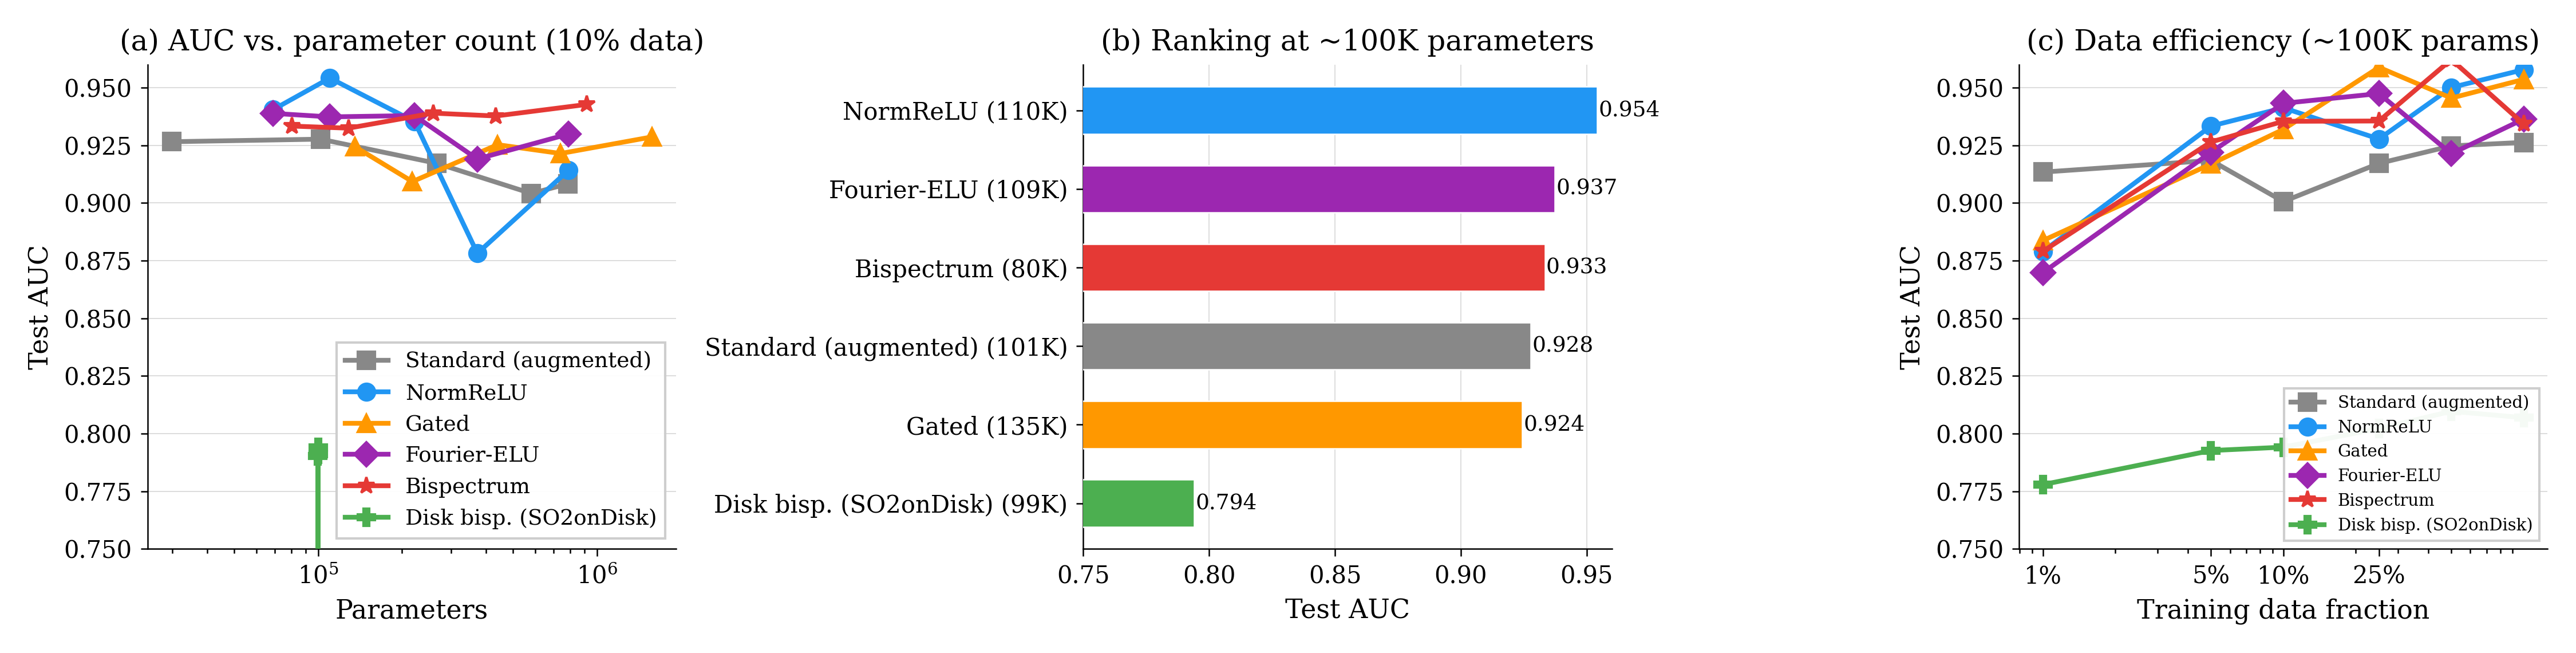
\includegraphics[width=\textwidth]{experiments/pcam/pareto_analysis.png}
  \caption{Pareto analysis of invariant pooling methods on PCam
    (10\% training data, seed 42).
    \textbf{(a)}~AUC vs.\ parameter count: bispectrum (red) shows the
    flattest curve, achieving consistently high AUC across all model
    sizes. Norm (blue) peaks sharply at $\sim$110k parameters then
    degrades.
    \textbf{(b)}~Head-to-head at $\sim$100k parameters: all equivariant
    models outperform the standard baseline when parameter counts are
    matched.
    \textbf{(c)}~Improvement from 1\% to 10\% training data at default
    architecture ($k{=}12$): bispectrum shows the largest absolute
    gain ($+$6.8pp).
    \textbf{(d)}~Ranking at $\sim$100k parameters.}
  \label{fig:pareto}
\end{figure}

\todo[inline]{Write $\sim$0.3 page interpreting the Pareto analysis. Cover:}
\begin{itemize}
  \item \textbf{Bispectrum is the most architecturally stable choice.}
    Its AUC varies by only $\sim$1pp across a 12$\times$ range of model
    sizes (80k--920k parameters), while norm swings by $>$7pp
    (0.878--0.954). For practitioners, bispectral pooling ``just works''
    without growth rate tuning.
  \item \textbf{At matched parameters ($\sim$100k), all equivariant
    models outperform the standard CNN.} Norm peaks at 0.954 AUC
    ($k{=}4$, 110k params), followed by Fourier-ELU (0.937),
    bispectrum (0.933), standard (0.928), and gate (0.924).
    The standard model's advantage in Table~\ref{tab:main-results}
    disappears once parameter counts are controlled.
  \item \textbf{Norm's instability across architectures is a practical
    concern.} Norm achieves the single best AUC (0.954) but its
    performance is highly sensitive to growth rate, dropping to 0.878 at
    $k{=}8$. This brittleness suggests that norm's completeness gap
    interacts unpredictably with model capacity.
  \item \textbf{Data scaling (panel c)}: all models improve
    substantially from 1\% to 10\% data. Bispectrum shows the largest
    absolute gain ($+$6.8pp), consistent with the hypothesis that
    complete invariants benefit more from additional data.
\end{itemize}


\subsection{Data-efficiency Pareto analysis}
\label{sec:exp-data-pareto}

To assess how each invariant pooling method utilises limited training
data, we fix per-model growth rates to match $\sim$100k parameters
(standard $k{=}12$, norm/Fourier-ELU $k{=}4$, gate $k{=}3$,
bispectrum $k{=}4$) and sweep the training set fraction from 1\% to
100\% (six log-spaced points, three seeds each).

\begin{figure}[h]
  \centering
  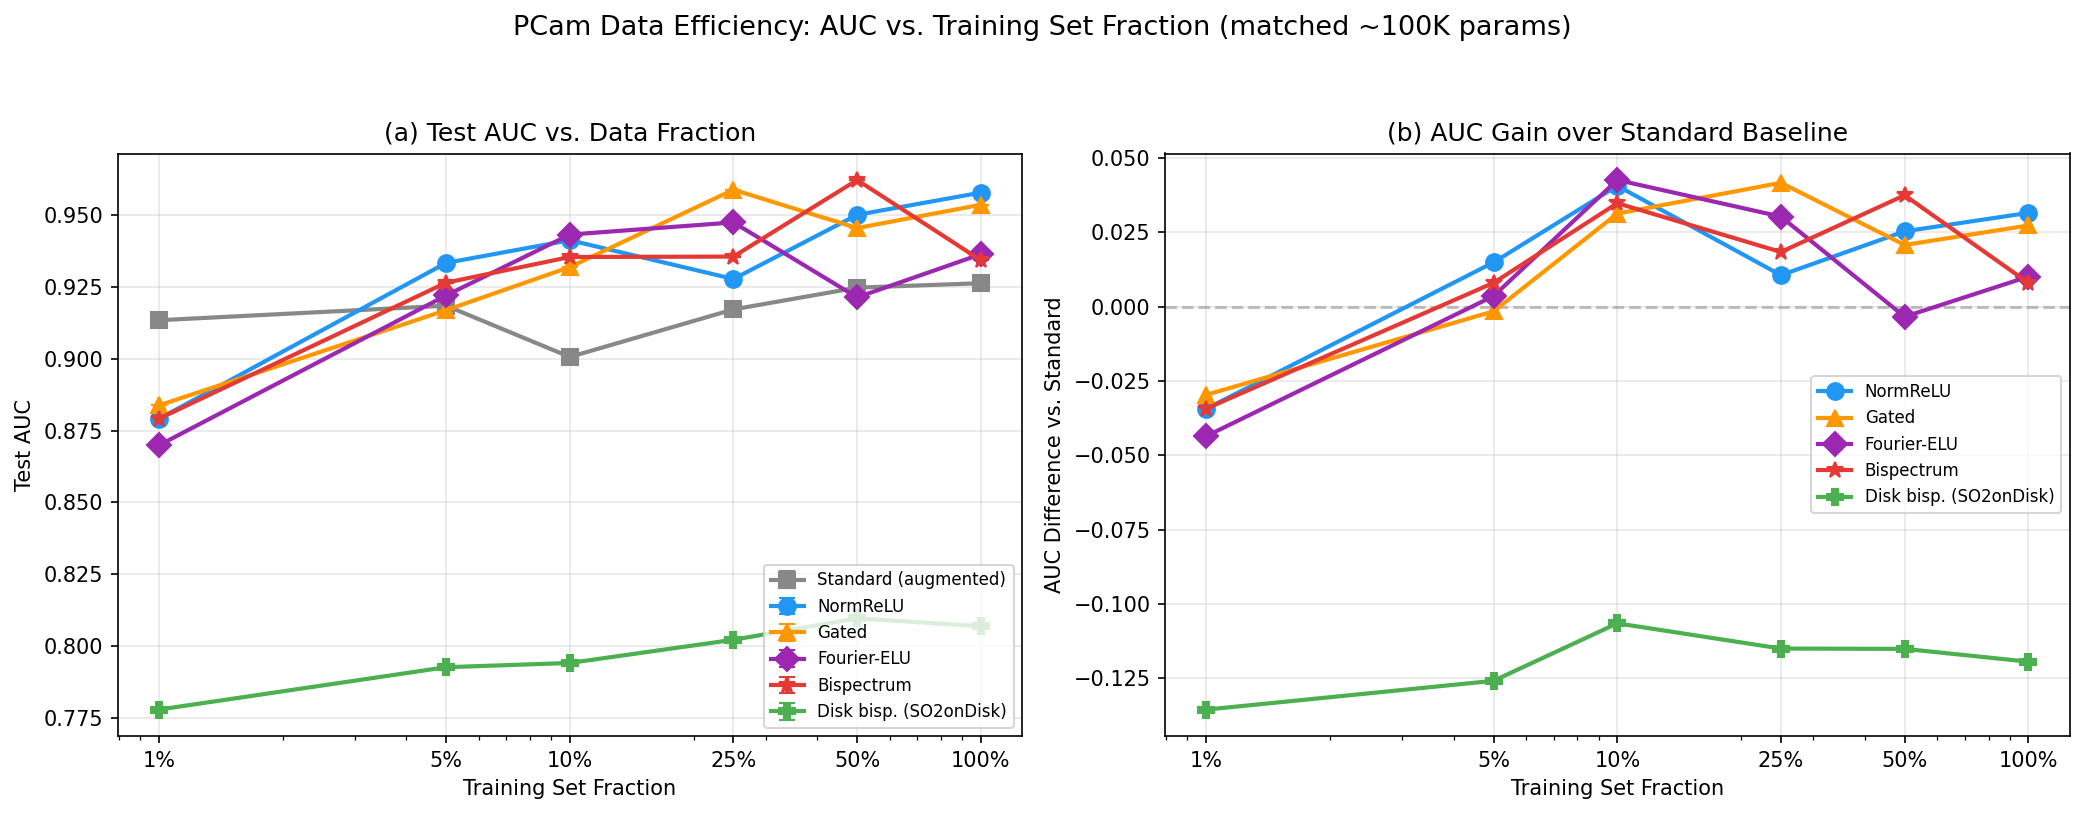
\includegraphics[width=\textwidth]{experiments/pcam/data_pareto_analysis.png}
  \caption{Data-efficiency Pareto analysis on PCam at matched
    $\sim$100k parameter budget.
    \textbf{(a)}~Test AUC vs.\ training set fraction (log scale) for
    five pooling methods; error bars show $\pm 1$ standard deviation
    over three seeds.
    \textbf{(b)}~AUC gain of each equivariant method relative to the
    standard (augmented) baseline at each data fraction.}
  \label{fig:data-pareto}
  \todo[inline]{Replace placeholder once sweep results are available.
    Run: \texttt{./run\_data\_pareto\_sweep.sh} then
    \texttt{python analyze\_data\_pareto.py}.}
\end{figure}

\todo[inline]{Write $\sim$0.3 page interpreting the data-efficiency
  Pareto analysis. Cover:}
\begin{itemize}
  \item Which pooling method achieves the highest AUC at small data
    fractions (1\%, 5\%)?
  \item At what data fraction do equivariant methods match or exceed
    the standard CNN?
  \item Does bispectral pooling show a steeper learning curve
    consistent with exact invariants requiring fewer samples?
\end{itemize}


\subsection{Bispectral contrastive regularization}
\label{sec:exp-contrastive}

\todo[inline]{Write $\sim$0.3 page. This experiment demonstrates the library
beyond invariant pooling---as a rotation-invariant regularizer.}

The bispectrum provides a natural contrastive signal: rotated copies of a
signal share identical bispectral coefficients by construction, so
$\|\betasel(f) - \betasel(T_g f)\| = 0$ without needing to track which
augmentation was applied.

\begin{itemize}
  \item \textbf{Dataset}: RotMNIST~\citep{cohen2016group}---MNIST digits
    rotated by arbitrary angles. 12k train / 50k test.
  \item \textbf{Baseline}: Standard CNN + supervised contrastive
    loss~\citep{chen2020simclr} using augmentation-labeled positive pairs.
  \item \textbf{Ours}: Same CNN + bispectral contrastive regularizer:
    $\mathcal{L}_{\text{bisp}} = \|\betasel(f_1) - \betasel(f_2)\|^2$
    for augmented pairs, added to the cross-entropy loss.
    Positive pairs are identified by bispectral distance rather than
    augmentation labels.
  \item \textbf{Metrics}: Test accuracy, rotation robustness
    ($\sigma_{\text{acc}}$ across rotation angles).
\end{itemize}

\begin{table}[h]
  \caption{RotMNIST results. Bispectral contrastive regularization provides
    rotation robustness without requiring augmentation labels.}
  \label{tab:contrastive-results}
  \centering
  \begin{tabular}{lcc}
    \toprule
    Model & Test Acc $\uparrow$ & Rot.\ $\sigma_{\text{acc}}$ $\downarrow$ \\
    \midrule
    Standard CNN              & {\color{red}XX.X\%} & {\color{red}X.XX} \\
    + augmentation            & {\color{red}XX.X\%} & {\color{red}X.XX} \\
    + supervised contrastive  & {\color{red}XX.X\%} & {\color{red}X.XX} \\
    + bispectral contrastive  & {\color{red}\textbf{XX.X\%}} & {\color{red}\textbf{X.XX}} \\
    \bottomrule
  \end{tabular}
\end{table}

\todo[inline]{Interpret results. The bispectral regularizer should provide
comparable or better rotation robustness to supervised contrastive learning,
without needing augmentation tracking. This demonstrates the library's
utility beyond invariant pooling.}


\section{Related Work}
\label{sec:related}

\todo[inline]{Write $\sim$0.75 page on related work. Frame comparisons in terms of what software/tools exist and what our library adds. Distinguish from each:}

\paragraph{Equivariant network libraries.}
\texttt{e2cnn}/\texttt{escnn}~\citep{weiler2019general, cesa2022program} provide steerable
convolution layers but no bispectral invariant pooling. The \texttt{bispectrum}
library is complementary: it provides the invariant map that
\texttt{escnn} lacks, and can be used as a drop-in replacement for
norm/gate pooling in existing architectures.

\paragraph{Bispectral neural networks.}
\citet{sanborn2023bispectral} propose learning the group from data using
bispectral features, but restrict to commutative groups and achieve lower
accuracy than equivariant baselines on RotMNIST (98.1\% vs.\ 99.3\% for E2CNN).%
\todo[inline,color=red!10]{Verify: 98.1\% BNN vs.\ 99.3\% E2CNN from Sanborn et al.\ Table~2.}
Our library handles non-abelian groups and integrates into existing
equivariant architectures rather than replacing them.

\paragraph{Bispectral CNNs.}
\citet{oreiller2022bispectral} introduce a bispectral U-Net for
medical image segmentation using SO(2) bispectra.
Their implementation is TensorFlow-based, uses the full (not selective)
bispectrum, and supports only SO(2).
Our library supports 7 group/domain pairs with selective coefficients,
GPU-accelerated PyTorch, and signal inversion.

\paragraph{CG product nonlinearities.}
Clebsch--Gordan Nets~\citep{kondor2018clebsch} and tensor field
networks~\citep{thomas2018tensor} use the CG tensor product as a nonlinearity.
While complete, the cost is $O(|G|^3)$ per layer.
The selective bispectrum achieves completeness at $O(|G|)$ coefficient cost
for finite groups, applied at the invariant pooling step.
The MACE symmetric contraction~\citep{batatia2024design} can be seen as a
generalized bispectrum; our work provides the selective reduction.

\paragraph{General SO(2) nonlinearities.}
\citet{franzen2021general} propose FFT $\to$ pointwise nonlinearity
$\to$ IFFT. This is approximate due to aliasing from harmonic truncation.
The bispectrum is exact by construction.

\paragraph{ML software at NeurIPS.}
Software papers at NeurIPS succeed when they pair engineering with
scientific contribution~\citep{paszke2019pytorch, gardner2018gpytorch,
ke2017lightgbm, moreau2022benchopt}. Our paper follows this template:
the library is the vehicle, and the steerable-to-Fourier bridge and
octahedral inversion resolution are the scientific contributions.

\paragraph{Tensor product expressivity.}
\citet{price2025freedom} systematically analyze the expressivity--runtime
tradeoff in equivariant tensor products, showing that faster variants
sacrifice expressivity. The selective bispectrum offers a complementary
perspective: it achieves completeness at $O(|G|)$ cost by leveraging the
algebraic structure of Kronecker products rather than approximating the
full tensor product.


\section{Discussion and Conclusion}
\label{sec:conclusion}

\todo[inline]{Write $\sim$0.75 page. Cover:}

\paragraph{Summary.}
We presented \texttt{bispectrum}, a PyTorch library that makes selective
$G$-bispectra practical as differentiable primitives for invariant feature
extraction, regularization, and signal reconstruction.
The library supports 7 group/domain pairs, provides GPU-accelerated
computation and signal inversion, and integrates into standard training
pipelines as a drop-in \texttt{nn.Module}.

Building the library required resolving two open problems:
the steerable-to-Fourier bridge (Theorem~\ref{thm:steerable-fourier})
that enables bispectral computation from non-abelian steerable features,
and the octahedral inversion gap that we resolved with bootstrap~+~LM
refinement. On PatchCamelyon, bispectral pooling achieves the highest
AUC among equivariant nonlinearities and the most stable Pareto frontier
across model sizes, while maintaining near-perfect rotation invariance.

\paragraph{Limitations.}
\begin{itemize}
  \item Selective $\SO(3)$ on $S^2$ remains an open problem---the library
    currently supports only the full bispectrum for this group.
  \item Inversion for continuous groups with band-limit truncation needs
    further study (stability under truncation).
  \item Broader empirical evaluation (cryo-EM, molecular ML) is future work.
\end{itemize}

\paragraph{Roadmap and governance.}
\todo[inline]{Write $\sim$3 sentences on roadmap. Cover:}
\begin{itemize}
  \item \textbf{Planned extensions}: selective $\SO(3)$ completeness (open
    mathematical problem), ball domain $S^2 \times \R^+$, integration with
    \texttt{escnn}/\texttt{e3nn}, applications to cryo-EM and
    molecular ML.
  \item \textbf{Maintenance}: MIT license, GitHub CI/CD with pre-commit hooks,
    pip-installable via \texttt{pip install bispectrum}, $>$90\% test coverage,
    Codecov integration.
  \item \textbf{Community}: hosted on GitHub
    (\texttt{geometric-intelligence/bispectrum}), issues and PRs welcome.
\end{itemize}


\begin{ack}
\todo[inline]{Add acknowledgments for camera-ready version. Include funding sources and competing interests.}
\end{ack}

\bibliographystyle{plainnat}
\bibliography{references}


\appendix

\section{Steerable-to-Fourier bridge: proof and practical consequences}
\label{app:proofs}

\todo[inline]{Insert full proof of P4 (steerable-to-Fourier bridge) here. Include:}
\begin{itemize}
  \item All supporting lemmas with proofs.
  \item The precise relationship between intertwiner coefficients
    and group Fourier matrices.
  \item The multi-head construction for representations that do not
    satisfy $m_i \geq d_i$.
\end{itemize}

\paragraph{Practical consequences for equivariant architectures.}
\todo[inline]{Discuss which escnn/e2cnn architectures satisfy the conditions of Theorem~\ref{thm:steerable-fourier}. Which standard configurations work out of the box? Which require modification (e.g., increasing multiplicity)?}

\paragraph{The BispectrumPool layer.}
\todo[inline]{Detail the concrete implementation:}
\begin{itemize}
  \item Receive equivariant features of shape $(B, C, |G|, H, W)$.
  \item Per channel, per spatial location: extract Fourier coefficients
    from the group dimension via group DFT.
  \item Compute selective bispectrum using the appropriate library module
    (\texttt{CnonCn} for $C_8$, \texttt{DnonDn} for $D_4$, etc.).
  \item Log-compress ($x \mapsto \mathrm{sign}(x) \cdot \log(1 + |x|)$)
    for numerical stability and project back via $1 \times 1$ convolution.
\end{itemize}


\section{Octahedral inversion: convergence analysis}
\label{app:octa-convergence}

\todo[inline]{Include convergence analysis for the bootstrap + LM inversion. Cover:}
\begin{itemize}
  \item Convergence plots: residual vs.\ iteration for representative signals.
  \item Multi-start statistics: fraction of initializations that converge
    to the correct orbit.
  \item Wall-clock timing breakdown: bootstrap init vs.\ LM iterations.
  \item Comparison with pure optimization (no bootstrap init) to show
    the value of the warm start.
\end{itemize}


\section{Extended benchmark tables}
\label{app:benchmarks}

\todo[inline]{Include full benchmark tables:}
\begin{itemize}
  \item Forward timing (CPU and GPU) for all modules at multiple group sizes.
  \item Inversion timing for all modules with inversion support.
  \item Memory usage (peak GPU memory) at various batch sizes.
  \item Hardware: report on at least 2 GPU types (e.g., A100 and V100).
\end{itemize}


\section{Experimental details}
\label{app:exp-details}

\todo[inline]{Include full experimental details:}
\begin{itemize}
  \item Architecture diagram of the equivariant DenseNet.
  \item Hyperparameter table (learning rate, weight decay, batch size,
    epochs, patience, growth rate, block config).
  \item Training curves (loss and AUC vs.\ epoch) for all models.
  \item Data augmentation details for the standard baseline.
  \item PCam data preprocessing: download from Zenodo, HDF5 loading,
    GPU-based augmentation pipeline.
\end{itemize}


\section{Additional experiments}
\label{app:additional-exp}

\todo[inline]{Include additional experiments if completed:}
\begin{itemize}
  \item Galaxy10 DECals: 10-class galaxy morphology classification.
  \item $D_4$ group results on PCam (dihedral instead of cyclic).
  \item Extended data efficiency curves with more training fractions.
\end{itemize}


\newpage
\input{checklist.tex}


\end{document}
